%% ----------------------------------------------------------------
%% InvestigationVision.tex
%% ---------------------------------------------------------------- 
\chapter{Investigation into Vision Algorithms} \label{Chapter:InvestigationVision}

\section{Comparison}
\inote{find some references to back these claims up}
%\inote{Talk about how to compare images and TEST them all. Make a final comparison to decide on which will be used}
In computer vision, there are many different ways of comparing two similar images. These include the sum of absolute differences (S.A.D.) (\cite{Hamzah:DistanceDetection}), the sum of squared differences (S.S.D.) and  normalised cross correlation (N.C.C.). Each of these methods will be explained and tested to compare them. All testing will use images seen in figure \ref{fig:StereoTest}. Each test uses the same size of image to compare to of 50$\times$ 50 pixels of the same part of the image. 

\begin{figure}
\centering
\subfigure[Left Image]{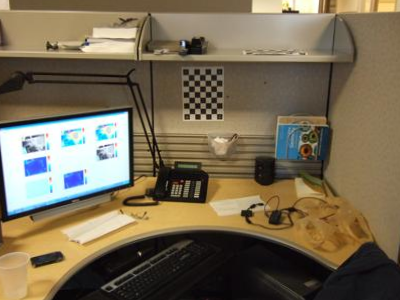
\includegraphics[scale=0.4]{./Figures/deskLeft.png} }
\subfigure[Right Image]{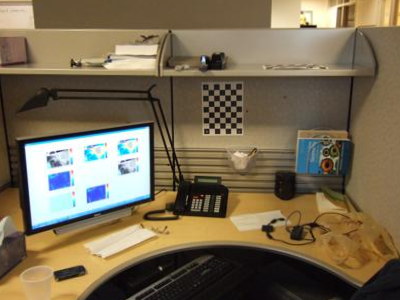
\includegraphics[scale=0.4]{./Figures/deskRight.png} }
\caption{Stereoscopic Test Images from MATLAB Examples}
\label{fig:StereoTest}
\end{figure}


%Explanation of how they work
\inote{Maybe do a basic 5x5 example for each?}
\subsection{Sum of Absolue Differences}

Given two indentically sized matricies, $A, B$ of dimensions $I,J$, SAD is defined as
\begin{equation} \label{eq:SAD}
SAD = \sum\limits_{i=0}^{I-1} \sum\limits_{j=0}^{J-1} A[i,j] - B[i,j] 
\end{equation}

This method takes each sub image and subtracts the observed sub image from the expected. All differences are then added together. This algorithm is simple and requires a small amount of computation. The algorithm returns values where a small result means the two images are well matched.

\subsection{Sum of Squared Differences}
\begin{equation}\label{eq:SSD}
SSD = \sum\limits_{i=0}^{I-1} \sum\limits_{j=0}^{J-1} (A[i,j] - B[i,j] )^2
\end{equation}

This is very similar to S.A.D. but adds more complexity by squaring each difference. This removes the ability of equally different but opposite differences cancelling each other out (grey to white of one pixel will cancel out a white to grey difference in the other). Again, a low result is a match in this case.

%\inote{sort chi out, if I want to do it...}
%\subsection{'Chi Squared'}
%$\chi ^{2}$ is ``Insert definition here". For use with images the equation can be adapted to \ref{eq:ChiSquare}. 
%
%\begin{equation} \label{eq:ChiSquare}
%\chi ^{2} = \sum\limits_{i=0}^{I-1} \sum\limits_{j=0}^{J-1}\frac{(A[i,j] - B[i,j])^2}{(A[i,j]+B[i,j])/2}
%\end{equation}


\subsection{NCC}
\begin{equation}\label{eq:NCC}
NCC =  \frac{1}{n}\sum\limits_{i,j} \frac{(A[i,j] - \bar{A}).(B[i,j] - \bar{B}}{\sigma _A . \sigma _B}
\end{equation}
\begin{center}
Where $n$ is the number of pixels in $A$ and $B$, \\$\sigma$ is the standard deviation of the image, and \\$\bar{A}$ is the a average pixel value. 
\inote{Find a source for this equation}
\end{center}
\inote{No date on Reference}
NCC is very similar to cross correlation, but normalised to reduce the error if one image is brighter than the other. It is common in computer vision (\cite{Tsai:NCC}) as cross correlation is a common operation in DSP so fast algorithms have been made to calculate this. 

Unlike S.S.D. and S.A.D., the normalised cross correlation gives a high value for a match. The downside to this algorithm comes with the complexity of the equation with division in it and a square root to calculate the standard deviation. These operations are rarely implemented in hardware and are time consuming to carry out. They also require floating point registers and operations slow on a Microcontroller with a small amount of floating point registers. 



%test and compare
\subsection{Comparison}

To compare these equations, a 50 by 50 image taken from the Right picture was compared with the left image over the entire valid range. The coordinates on the graph give the centre pixel of the calculation. Fi

\begin{figure}
\centering
\subfigure[S.A.D Results (Low match)\label{fg:Results:SAD}]{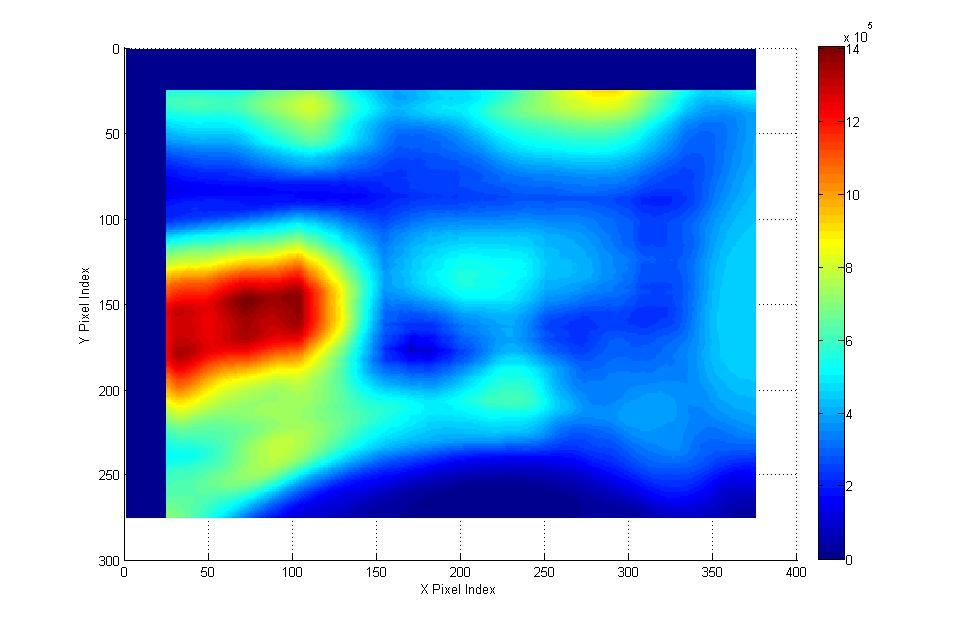
\includegraphics[width = 12cm, keepaspectratio]{./Figures/SADResults.jpg} }
\subfigure[S.S.D. Results (Low match)\label{fg:Results:SSD}]{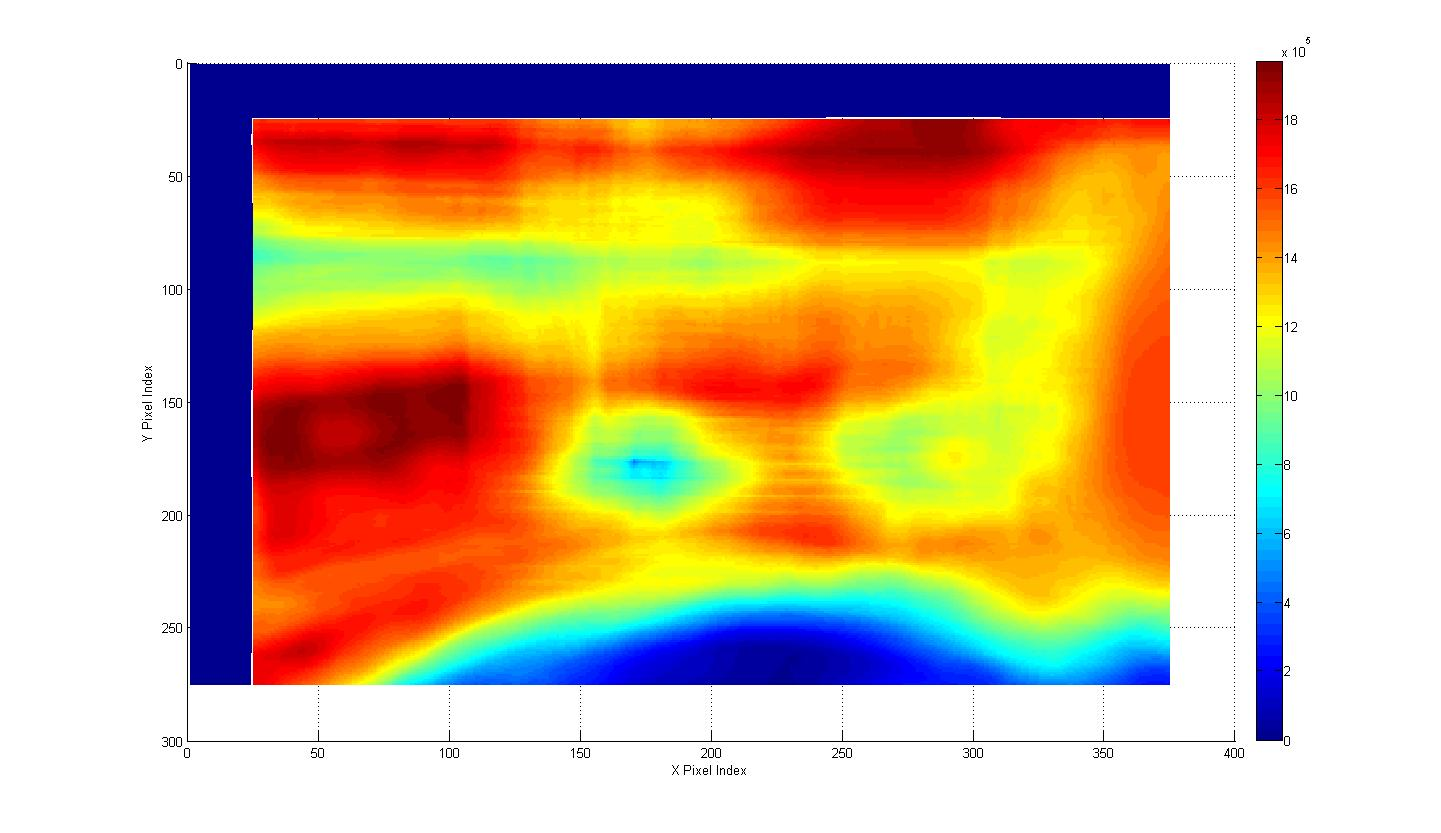
\includegraphics[width = 12cm, keepaspectratio]{./Figures/SSDResults.jpg} }
\subfigure[N.C.C. Results (High match)\label{fg:Results:NCC}]{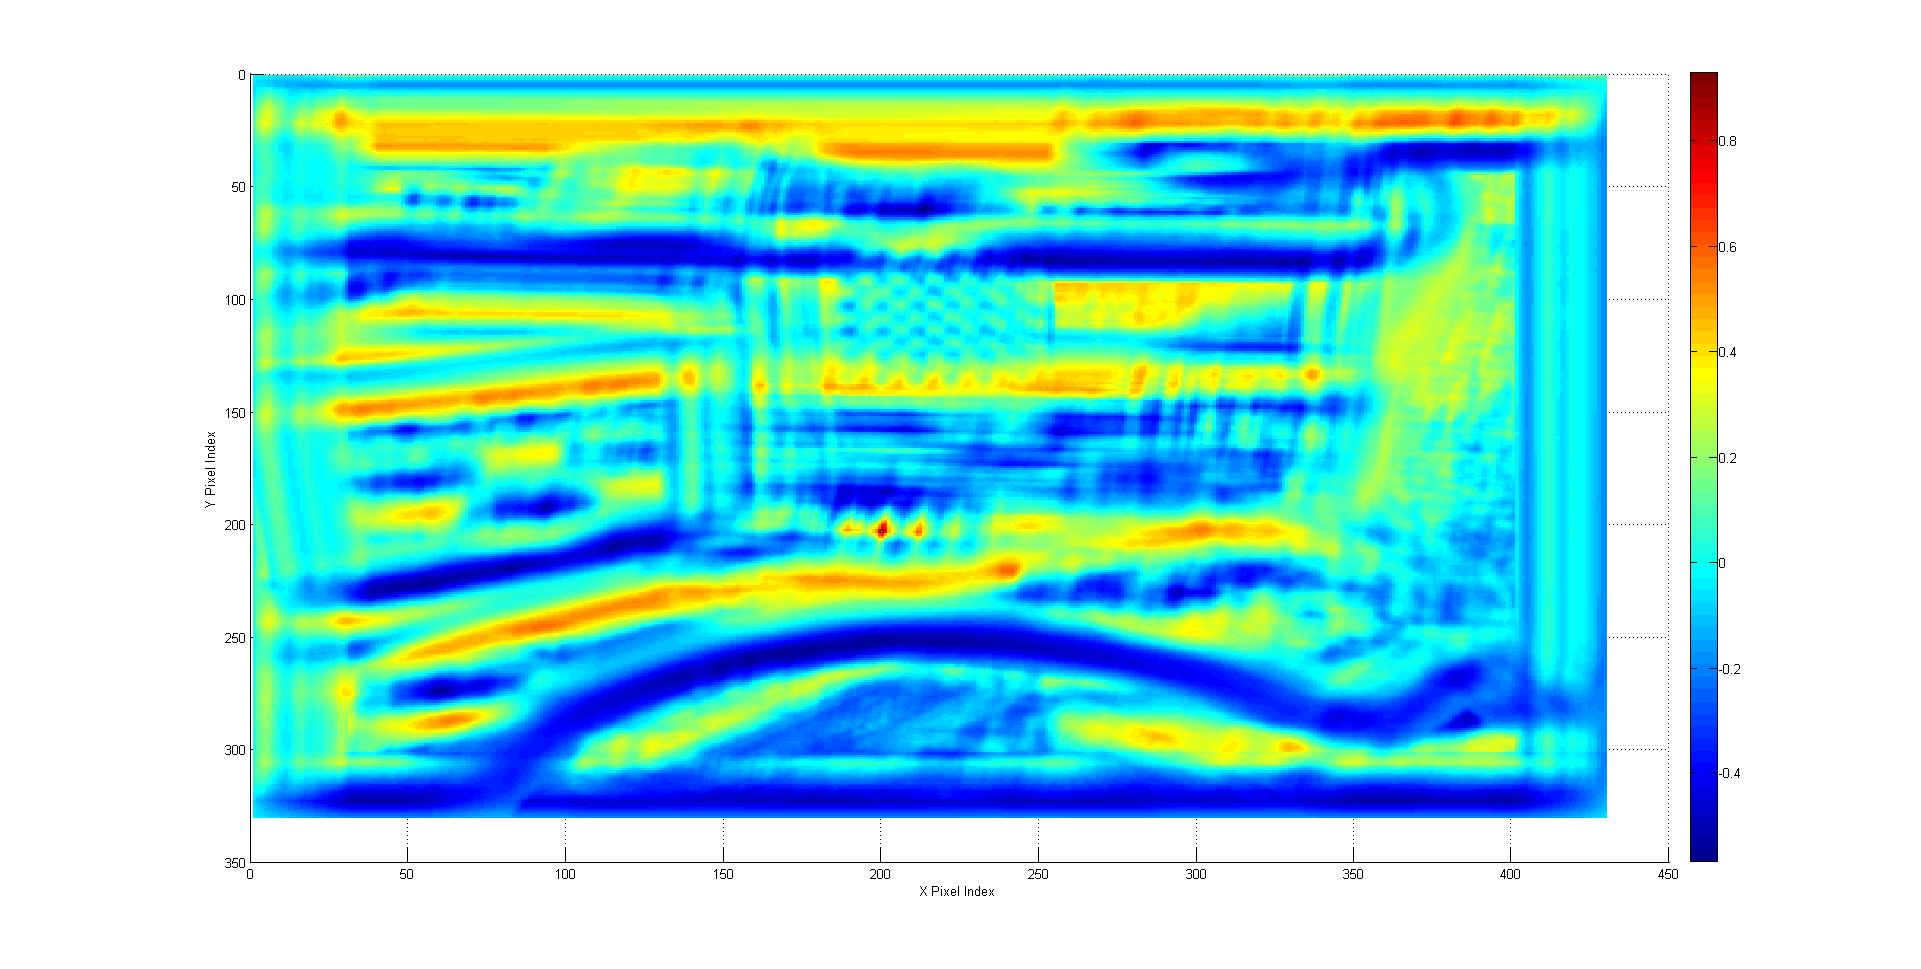
\includegraphics[width = 12cm, keepaspectratio]{./Figures/NCCResults.jpg} }
\caption{Result Graphs of Comparison Algorithms}
\label{fg:CompResults}
\end{figure}

Each of the graphs show the correct area being indentified as a match, but this also highlights the downfalls of the SAD and SSD. The figures in figure \ref{fg:CompResults} are orientated to match the orientation of the images in figure \ref{fig:StereoTest}. Each of the images is tested by attempting to match the phone from the test figure. The actual match should be around $(170, 176)$. An exact result cannot be estimated as the images are not matched perfectly - there isn't an exact integer of pixel difference between the images. This is the sub pixel problem.
\inote{reference for sub pixel problem?}

SAD results in figure \ref{fg:Results:SSD} show large areas of matching. The actual match is at (170, 175) and a minimum does occur at this position as expected of a value of $5.66\times 10^4$. However, along the bottom of the image where a dark area occurs in the lower part of figures \ref{fig:StereoTest} below the desk, the SAD algorithm detects a greater comparison with the lowest value in this area being $3370$ at $(227, 275)$. This creates a false detection here. 

SSD shows matches in the same two areas: where a match should occur and the dark area beneath the desk. The minimum values where the match should occur is $4.355 \times 10^5$ at location $(170,176)$. However, again, there is thought to be a large match correlation between the dark area under the desk where the actual lowest value of $2.768$ is at $(225,274)$. This, again, is a false match and is a downfall of this algorithm. 

The NCC results are visible in figure \ref{fg:Results:NCC}. A match can be seen at coordinate $(195,201)$ with a peak value of $0.9654$. The coordinate is different to the previous results because the cross correlation works over the boundary of the image creating more results. The dimensions of the image are 300 $\times$ 400, but the NCC returns an data set of dimensions 350 $\times$ 450 when using a box size of 50 $\times$ 50. To get the actual match, half of the box size must be subtracted from the returned coordinate. This means the match occurs at $(170,176)$. 

\subsection{Conclusion}
It can be seen there is a direct correlation between the complexity of the matching algorithm to the reliability of the match returned. In brightly lit, colourful environments absent of dark colours, SAD and SSD should provide a reliable result, but this cannot guaranteed to always be the case. Therefore further development of the matching algorithm will start with using the Normalised Cross Correlation. There is a compromise of complexity for reliability, of which reliability is more desirable. Cross correlation is also a large area of research, so optimised algorithms do exist. 

\section{Range Finding}
\inote{Derive the range finding equations and test them}

\subsection{Derivations}

By using two images separated by a horizontal difference, the range of an object can be found given some characteristics of the camera. The following is a derivation of the equations used to calculate distance. 

The problem is broken down into 3
\begin{enumerate}
\item Object is between the cameras (Figure \ref{problem_between})
\item Object is directly in front of a camera
\item Object is in left or right hand sides of both images
\end{enumerate}

\begin{figure}
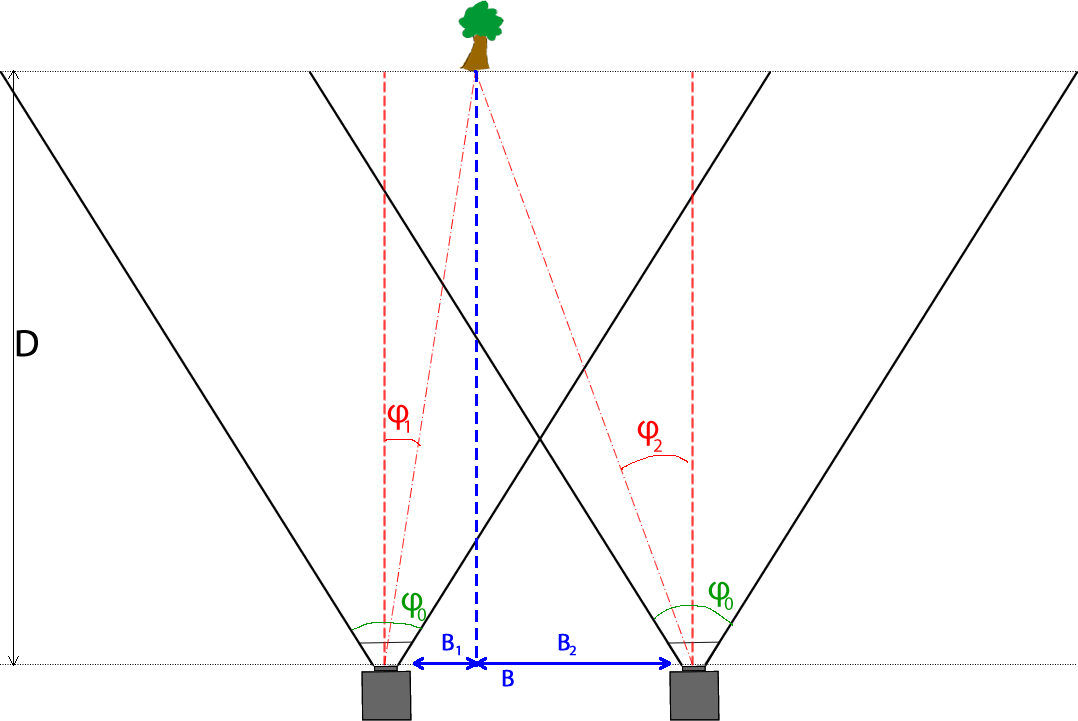
\includegraphics[width=\textwidth,height=\textheight,keepaspectratio]{Figures/problem1.png}
\caption{Problem 1 - Object is between the Cameras}
\label{problem_between}
\end{figure}

\subsubsection{Object is between the Cameras}
Derivation from \cite{Mrovlje:Distance_Stereoscopic}.
\begin{equation} \label{eq:B}
B = B_{1} + B_{2} = D\tan(\varphi_{1}) + D\tan(\varphi_{2})
\end{equation}

\begin{equation} \label{eq:D}
D = \frac{B}{\tan(\varphi_{1}) + \tan(\varphi_{2})}
\end{equation}


\begin{figure}
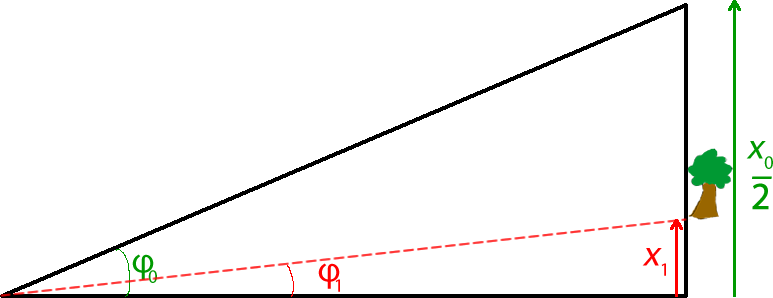
\includegraphics[width=\textwidth,height=\textheight,keepaspectratio]{Figures/left_simplified.png}
\caption{Problem 1 : Left Camera Simplified}
\label{Left_Simplified}
\end{figure}

\begin{equation} \label{eq:phi}
D\tan(\frac{\varphi_{0}}{2}) = x_{0} / 2
\end{equation}

\begin{equation} \label{eq:phi1}
D\tan(\varphi_1) = x_1
\end{equation}

Dividing \eqref{eq:phi1} by \eqref{eq:phi}

\begin{equation} \label{eq:tanovertan}
\frac{\tan(\varphi_1)}{\tan(\frac{\varphi_0}{2})} = \frac{2x_1}{x_0}
\end{equation}

\begin{equation} \label{eq:phionesolved}
\tan(\varphi_1) = \frac{2x_1\tan(\frac{\varphi_0}{2})}{x_0}
\end{equation}

It can also be shown that for the right camera:

\begin{equation} \label{eq:phitwosolved}
\tan(\varphi_2) = \frac{-2x_2\tan(\frac{\varphi_0}{2})}{x_0}
\end{equation}

Substitution equations \eqref{eq:phionesolved} and \eqref{eq:phitwosolved} into \eqref{eq:D} gives

\begin{equation} \label{eq:Distance1}
D = \frac{Bx_0}{2\tan(\frac{\varphi_0}{2})(x_1 - x_2)}
\end{equation}


\subsubsection{Object is to the same side in each camera}
Derivation is based on the derivation from \cite{DistanceEstimation}. Using figure \ref{problem_toleft}:

\begin{equation} \label{eq:p2:tanphi1}
D.\tan(\varphi_{1}) = x_{1}
\end{equation}

\begin{equation} \label{eq:p2:tanphi0}
D.\tan(\frac{\varphi_{1}}{2}) = \frac{x_{0}}{2}
\end{equation}

\begin{equation} \label{eq:p2:tanphi0and1}
\frac{\tan(\varphi_{1})}{\tan(\frac{\varphi_0}{2})} = \frac{2x_1}{x_0}
\end{equation}

\begin{equation} \label{eq:p2:phi1}
\varphi_1 = \arctan(\frac{2x_1}{x_0}\tan(\frac{\varphi_0}{2})
\end{equation}

and similarly
\begin{equation} \label{eq:p2:phi2}
\varphi_2 = \arctan(\frac{2x_2}{x_0}\tan(\frac{\varphi_0}{2})
\end{equation}
\begin{equation} \label{eq:p2:theta}
\theta = \varphi_2 - \varphi_1
\end{equation}

Using the sine equality rule:

\begin{equation} \label{eq:p2:sineeq}
\frac{R}{\sin(\frac{\pi}{2} - \varphi_2)} = \frac{B}{\sin(\theta)}
\end{equation}

\begin{equation} \label{eq:p2:R}
R = B.\frac{\sin(\frac{\pi}{2} - \varphi_2)}{\sin(\theta)} = B \frac{\cos(\varphi_2)}{\sin(\theta)}
\end{equation}

\begin{equation} \label{eq:p2:DeqR}
D = \cos(\varphi_1).R
\end{equation}
Substituting \eqref{eq:p2:theta} into \eqref{eq:p2:R}, and then into \eqref{eq:p2:DeqR}:

\begin{equation} \label{eq:p2:DeqB}
D = B.\frac{\cos(\varphi_2).\cos(\varphi_1)}{sin(\varphi_2 - \varphi_1)}
\end{equation}

Where $\varphi_1$ is defined in equation \eqref{eq:p2:phi1} and $\varphi_2$ is defined in equation \eqref{eq:p2:phi2}. 

\begin{figure}
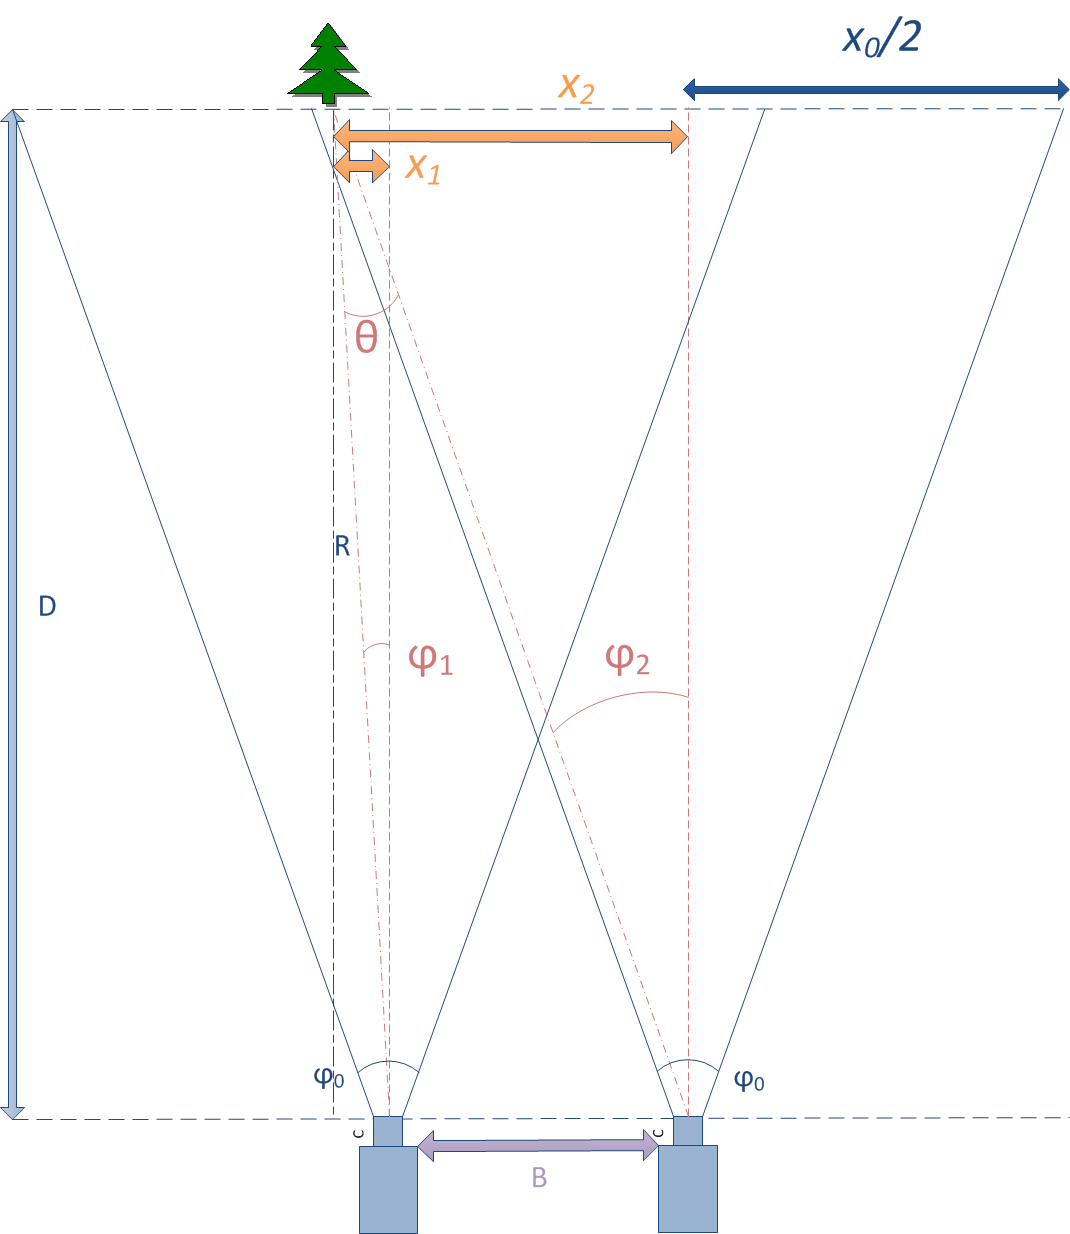
\includegraphics[width=\textwidth,height=\textheight,keepaspectratio]{Figures/problem2.png}
\caption{Problem 2 - Object is to the same side in both cameras}
\label{problem_toleft}
\end{figure}

\subsubsection{Object is in front of a camera}
The distance, $D$, in this problem is given by:

\begin{equation} \label{eq:p3:D}
D = B \tan(\frac{\pi}{2} - \varphi_{2})
\end{equation}
Where $\varphi_2$ can be found from equation \ref{eq:p2:phi2}. 
\begin{figure}
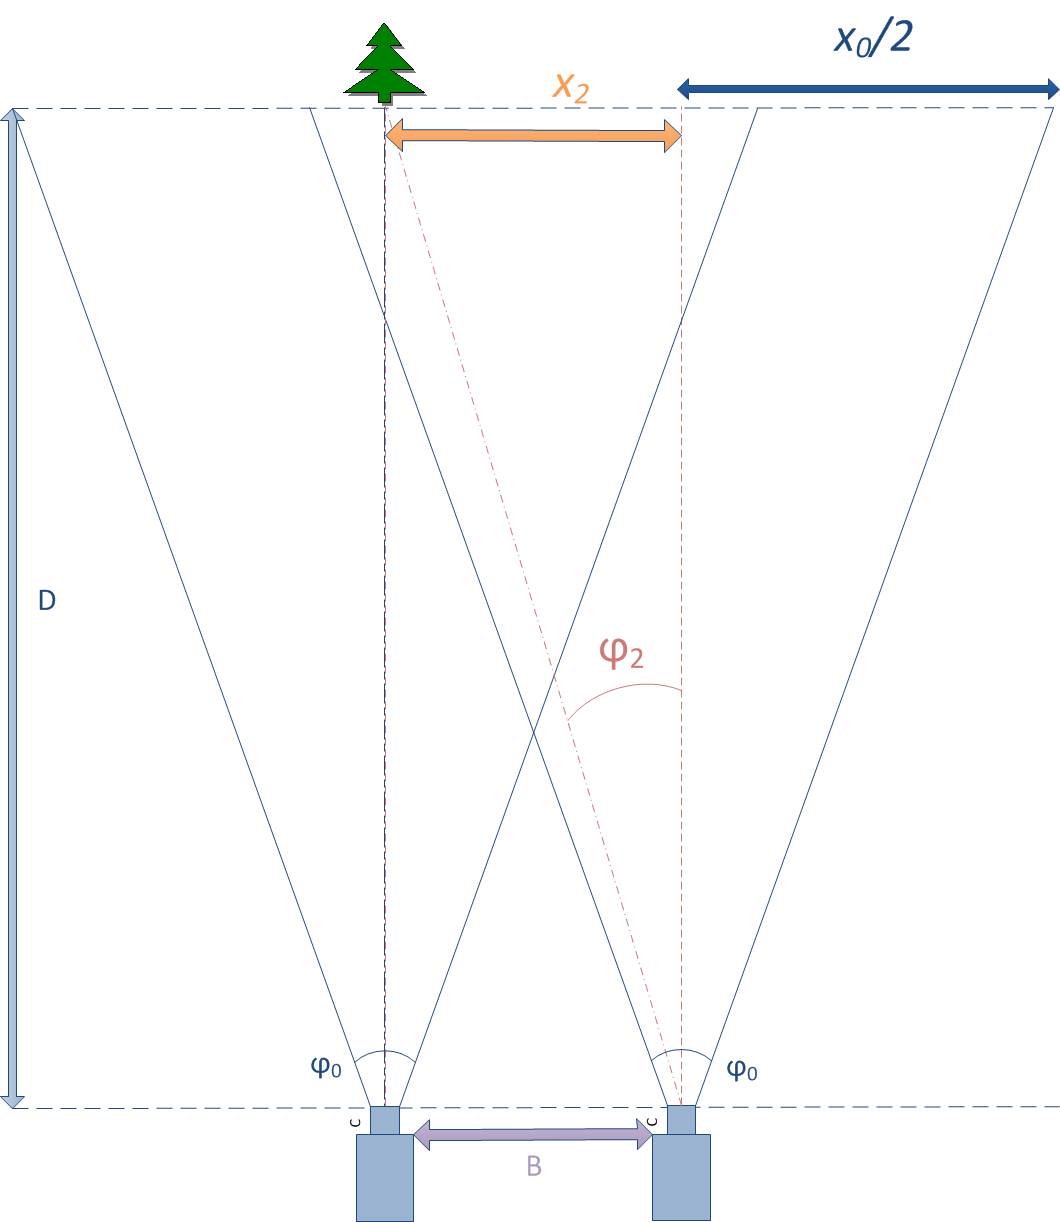
\includegraphics[width=\textwidth,height=\textheight,keepaspectratio]{Figures/problem3.png}
\caption{Problem 3 - Object is directly in front of a camera}
\label{fig:problem_infront}
\end{figure}

\subsubsection{Summary}
There are three situations that can occur. These are listed below with their equations.

Object is between the two cameras:
\begin{equation} \label{eq:summary:1}
D = \frac{Bx_0}{2\tan(\frac{\varphi_0}{2})(x_1 - x_2)}
\end{equation}

Object is to the same side in both images:
\begin{equation} \label{eq:summary:2}
D = B.\frac{\cos(\varphi_2).\cos(\varphi_1)}{sin(\varphi_2 - \varphi_1)}
\end{equation}
Object is directly in front of a camera:
\begin{equation} \label{eq:summary:3}
D = B \tan(\frac{\pi}{2} - \varphi_{2})
\end{equation}

Where $\varphi_1$ is defined in equation \eqref{eq:p2:phi1} and $\varphi_2$ is defined in equation \eqref{eq:p2:phi2}.